%-----------------------------------------------------------------------------%
\chapter{\babDua}
%-----------------------------------------------------------------------------%
Pada bab ini akan dibahas mengenai kajian pustaka yang diambil dari penelitian- penelitian sebelumnya yang relevan. Kajian pustaka ini selanjutnya akan digunakan sebagai landasan dalam melakukan penelitian ini.

%-----------------------------------------------------------------------------%
\section{\SCM (\scm) atau Manajemen Rantai Pasok}
%-----------------------------------------------------------------------------%
Supply chain (rantai pengadaan) adalah suatu sistem melalui mana suatu organisasi itu menyalurkan barang produksi dan jasanya kepada para pelanggannya. Rantai ini juga merupakan jaringan atau jejaring dari berbagai organisasi yang saling berhubungan yang mempunyai tujuan yang sama yaitu sebaik mungkin menyelenggarakan pengadaan atau penyaluran barang tersebut. Kata penyaluran mungkin kurang tepat karena dalam istilah supply termasuk juga proses perubahan barang tersebut jadi misalnya dari bahan mentah menjadi barang jadi.\cite{Manajemen}

\scm merupakan rangkaian kegiatan perencanaan, koordinasi, dan pengendalian seluruh proses bisnis dan aktivitas dalam supply chain untuk menciptakan consumer value terbaik dengan biaya yang efisien namun tetap memenuhi seluruh kebutuhan stakeholder lain dalam supply chain \cite{Hilman2013}. \SCM (\f{SCM}) merupakan bidang kajian yang terletak pada efisiensi dan efektifitas aliran barang, informasi dan aliran uang yang terjadi secara simultan sehingga dapat menyatukan supply chain management dengan pihak yang terlibat \cite{Vistasusiyanti2017}. \SCM adalah koordinasi dari semua aktivitas supply pada suatu organisasi dari supplier dan partner ke konsumennya \cite{Hayati2015a}.

Berdasarkan dari beberapa definisi di atas maka dapat disimpulkan bahwa \scm merupakan suatu sistem rangkaian kegiatan perancanaan, koordinasi, dan pengandalian seluruh proses bisnis dan aktivitas supply pada suatu organisasi dari supplier ke partner ke konsumen serta juga merupakan bidang kajian yang terletak pada efisiensi dan efektifitas aliran barang informasi dan aliran uang yang terjadi secara simultan.


%-----------------------------------------------------------------------------%
\section{Konsep \SCM}
%-----------------------------------------------------------------------------%
Dari definisi \SCM maka dapat dikatakan \f{logistics network} (Hubungan logistik\footnote{Berasarkan kamus KBBI:pengadaan, perawatan, distribusi, dan penyediaan (untuk mengganti) perlengkapan, perbekalan, dan ketenagaan;}) dalam hubungan ini beberapa pemain utama yang merupakan perusahaan-perusahaan yang mempunyai kepentingan yang sama tersebut yaitu\cite{Manajemen}:
\begin{itemize}
	\item \f{suppliers}
	\item \f{manufacturer}
	\item \f{distribution}
	\item \f{retail outlets}
	\item \f{customers}
\end{itemize}
\bo{Chain 1: Suppliers} \\
Jaringan bermula dari sini, dimana merupakan sumber yang menyediakan bahan pertama dimana mata rantai penyaluran barang akan bermulai. Bahan pertama ini dapat dalam bentuk bahan baku, bahan mentah, bahan penolong, bahan dagangan, suku cadang dan sebagainya. Jumlah supplier bisa banyak ataupun sedikit.\\ \\
\bo{Chain 1-2: Suppliers} $\to$ \bo{Manufacturer} \\
Rantai pertama dihubungkan dengan rantai ke dua yaitu \f{'manufacturer'} atau \f{plants} atau \f{assembler} atau \f{fabricator} atau bentuk lain yang melakukan pekerjaan membuat, memfabrikasi, mengasembling, merakit, mengkonversikan ataupun menyelesaikan barang (finishing). Hubungan konsep
\f{supplier partnering} antara manufaktur dengan \f{supplier} mempunyai potensi yang menguntungkan bagi kedua belah pihak. Dengan konsep ini, manufaktur sudah memiliki perjanjian atau kontrak dengan supplier sehingga terdapat kepastian harga produk untuk sebagai \f{supplier} dan kepastian kuantitas dan kualitas produk untuk pengolah sebagai manufaktur.\\ \\
\bo{Chain 1-2-3: Suppliers} $\to$ \bo{Manufacturer} $\to$ \bo{Distribution}\\
Barang yang sudah jadi yang sudah dihasilkan oleh manufacturer sudah mulai harus disalurkan kepada pelanggan. Walaupun tersedia banyak cara untuk penyaluran barang ke pelanggan, yang umum adalah melalui distributor dan ini biasanya ditempuh oleh sebagian besar supply chain. Barang dari pabrik melalui gudangnya disalurkan kepada gudang distributor atau wholesaler atau pedagang besar dalam jumlah besar dan pada waktunya nanti pedagang besar menyalurkan dalam jumlah yang lebih kecil kepada retailers atau pengecer.\\ \\
\bo{Chain 1-2-3-4: Supplier $\to$ Manufacturer $\to$ Distribution $\to$ Retail Outlets}\\
Pedagang besar biasanya mempunyai fasilitas gudang sendiri atau dapat juga menyewa dari pihak lain. Gudang ini digunakan untuk menimbun barang sebelum disalurkan lagi ke pihak pengecer. Sekali lagi disini ada kesempatan untuk memperoleh penghematan dalam bentuk jumlah inventories dan biaya gudang dengan cara melakukan desain kembali pola-pola pengiriman barang baik dari gudang manufacturer maupun kepada toko pengecer (retail outlets). \\ \\
Walaupun ada beberapa pabrik yang langsung menjual barang hasil produksinya kepada pelanggan, namun secara relatif jumlahnya tidak banyak dan kebanyakan menggunakan pola seperti di atas.\\ \\
\bo{Chain 1-2-3-4-5 : Supplier $\to$ Manufacturer $\to$ Distribution $\to$ Retail Outlets $\to$ Customers}\\
Para pengecer atau retailers ini menawarkan barangnya langsung kepada para pelanggan atau pembeli atau pengguna barang tersebut. Dalam pengertian outlets ini termasuk toko, warung, department store, super market, toko koperasi, mal, club stores dan sebagainya pokoknya dimana pembeli akhir melakukan pembelian.

Dari penjelasan pelaku-pelaku supply chain tersebut di atas, dapat dikembangkan suatu model supply chain, yaitu suatu gambaran plastis mengenai hubungan mata rantai dari pelaku-pelaku tersebut yang dapat berbentuk seperti mata rantai yang terhubung satu dengan yang lain. Model supply chain dikembangkan dengan cukup baik pada tahun 1994 oleh A.T.Kearney seperti tertera dan dapat dilihat dalam Gambar \pic~\ref{fig:modelSCM} berikut:
\begin{figure}
	\centering
	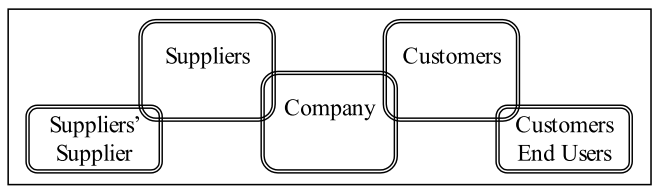
\includegraphics[width=0.80\textwidth]
		{pics/model_scm.png}
	\caption{Model \SCM}
	\label{fig:modelSCM}
\end{figure}

Dalam ilustrasi ini, \f{suppliers' suppliers} telah dimasukkan untuk menunjukkan hubungan yang lengkap dari sejumlah perusahaan atau organisasi yang bersama-sama mengumpulkan/mencari, merubah dan mendistribusikan barang dan jasa kepada pelanggan terakhir. Salah satu faktor kunci (key factor) untuk mengoptimalisasikan supply chain ialah dengan menciptakan alur informasi yang bergerak secara mudah dan akurat diantara jaringan atau mata rantai tersebut dan pergerakan barang yang efektif dan efisien yang menghasilkan kepuasan maksimal pada para pelanggan. 

%-----------------------------------------------------------------------------%
\section{Metode \f{Lot Sizing}}
%-----------------------------------------------------------------------------%
Dalam proses pengendalian persediaan barang terdapat beberapa metode \f{lotting} yang dapat digunakan. Proses \f{lotting} adalah suatu proses untuk menentukan besarnya pesanan individu yang optimal berdasarkan pada hasil perhitungan kebutuhan bersih \cite{Ibrahim}. Banyak alternatif dalam menentukan ukuran \f{lot}. Beberapa teknik untuk menambahkan ongkos pengiriman dan ongkos simpan, atau juga dengan konsep jumlah pemesanan tetap atau dengan periode pemesanan tetap. Dengan menentukan model \f{lot sizing} yang tidak tepat mengakibatkan jumlah persediaan tidak sesuai dengna kebutuhan yang sebenarnya, kelebihan persediaan juga berdampak pada meningkatnya biaya yang di timbulkan akibat barang yang masih belum terjual (tersimpan) dan mengurangi profitibilitas sebagai hasil dari penambahan modal kerja, asuransi, pajak dan keusangan. Kekurangan persediaan mengakibatkan tidak dapat memenuhi kebutuhan konsumen dan ketidak puasan konsumen akan terjadi dan mengakibatkan kehilangan kesempatan memperoleh keuntungan yang seharusnya di dapatkan.

Berikut ini beberapa metode \f{lot sizing} di antaraya sebagai berikut \cite{Almahdy}:
\begin{enumerate}
	\item \bo{\f{Lot For Lot (LFL)}}\\
	Teknik ini merupakan teknik lot sizing yang paling sederhana dan mudah dimengerti. Pemesanan dilakukan dengan pertimbangan minimasi ongkos simpan. Pada teknik ini, pemenuhan kebutuhan bersih (Rt) dilaksanakan di setiap periode yang membutuhkannya, sedangkan besar ukuran kuantitas pemesanannya (lot size) adalah sama dengan jumlah kebutuhan bersih yang harus dipenuhi pada periode yang bersangkutan. Teknik ini biasanya digunakan untuk item-item yang mahal atau yang tingkat kontinuitas permintaannya tinggi.
	
	\item \bo{\f{Fixed Order Quantity (FOQ)}}\\
	FOQ adalah sistem persedian probalistik yang variabel keputusan menggunakan Q (menotasikan kuantitas) pesanan tetap yang optimal. Kriteria optimal adalah total biaya persediaan yang minimal (Baroto, 2002). Tujuan persediaan dengan metode ini adalah untuk menentukan jumlah pesanan yang paling optimal dengan biaya yang minimal dan titik pemesanan kembali (reorder point). Prinsip FOQ atau pengendalian persediaan sistem Q adalah pemesanan dilakukan pada saat mencapai batas titik pemesanan (reorder point). Jumlah masing-masing unit produk yang dipesan sudah tetap. Namun pemesanannya dapat berbeda waktunya (kapan reorder point dapat tercapai). Jumlah persediaan yang menjadi kebutuhan selama waktu ancang-ancang dengan memperhitungkan kebutuhan yang berfluktuasi selama waktu ancang-ancang tersebut. Persediaan untuk meredam fluktuasi ini dinamakan persediaan pengaman (Tersine, 1994). Dapat dikatakan Safety stock dalam FOQ system, diperlukan untuk mengatasi adanya fluktuasi demand selama lead time. Safety stock untuk demand probabilistik dengan stockout case lost sales dimana demand yang tidak dapat dipenuhi akan dianggap hilang.
	
	\item \bo{\f{Economic Order Quantity ( EOQ )}}\\
	Russel dan Taylor (2003) menyatakan bahwa model EOQ digunakan untuk menentukan kuantitas pesanan persediaan yang meminimumkan biaya langsung penyimpanan persediaan dan biaya pemesanan persediaan. Menurut Rangkuti (2002), Model EOQ dapat diterapkan apabila asumsi-asumsi berikut ini dipenuhi:
	
	\begin{enumerate}
		\item Permintaan akan produk adalah konstan, seragam dan diketahui
		\item Harga per unit produk adalah konstan
		\item Biaya penyimpanan per unit per tahun konstan
		\item Biaya pemesanan per pesanan konstan
		\item Waktu antara pesanan dilakukan dan barang-barang diterima konstan
		\item Tidak terjadi kekurangan bahan atau back orders Rumus EOQ yang bisa digunakan adalah \equ~\ref{eq:eoqRumus} berikut:
		
		\noindent \begin{align}\label{eq:eoqRumus}
			EOQ &= \sqrt{\frac{2DS}{H}}
		\end{align}\\
		Dimana:\\
		D = Kebutuhan bahan selama satu periode\\
		S = Biaya persiapan/pemesanan setiap kali pesan\\
		H = Biaya penyimpanan per unit\\
		Setelah diperoleh nilai kuantitas pesanan optimal dengan teknik EOQ, maka model MRP dapat dilakukan dengan melakukan pesanan sebesar kelipatan dari EOQ yang lebih besar dan terdekat dengan kebutuhan bersih.
		
	\end{enumerate}

	\item \bo{\f{Period Order Quantity ( POQ )}}\\
	Teknik POQ disebut juga dengan Economic Time CycIe. Teknik POQ ini digunakan untuk menentukan interval waktu order (Economic Order Interval). Keuntungan menggunakan teknik POQ adalah dapat menghasilkan lot size order yang berbeda dalam memenuhi net requirement. Teknik POQ ini akan lebih baik kemampuannya jika digunakan pada saat biaya setup tiap tahun sama tetapi biaya carryingnya lebih rendah, (Imam, 2005).
\end{enumerate}

Pada penelitian ini metode \f{lot sizing} yang akan digunakan adalah metode \f{EOQ} berdasarkan asumsi-asumsi kajian yang telah di temukan dari penelitian sebelumnya. Metode \f{EOQ} dapat digunakan apabila pola permintaan kebutuhan bersifat terus menerus dan tingkat kebutuhan yang konstan \cite{Ibrahim, Fuad}. Metode tersebut sesuai dengan proses bisnis yang sedang berjalan.

%-----------------------------------------------------------------------------%
\section{\f{ROP (Reorder Point)}}
%-----------------------------------------------------------------------------%
Reorder point adalah sebuah titik dimana suatu pesanan baru harus dilakukan (atau persiapan dimulai). Hal ini juga di pengaruhi oleh lead time, yaitu waktu yang dibutuhkan untuk menerima kuantitas pesanan setelah pesanan dilakukan atau persiapan dimulai.

Berikut ini cara untuk mendapatkan nilai reorder point pada \equ~\ref{eq:ropRumus} \cite{Ibrahim}:
\noindent \begin{align}\label{eq:ropRumus}
	ROP &= Q \times Lt
\end{align}\\
Keterangan:\\
Q = Jumlah tingkat kebutuhan\\
Lt = Lead time

%-----------------------------------------------------------------------------%
\section{\f{Safety Stock}}
%-----------------------------------------------------------------------------%
Persediaan Pengaman (Safety stock) muncul ketika apotek dihadapkan dengan ketidakpastian akan permintaan obat sehingga akan ada kemungkinan kehabisan stok.

Untuk itu perhitungan safety stock adalah sebagai berikut \equ~\ref{eq:safeStockRumus} \cite{Ibrahim}:
\noindent \begin{align}\label{eq:safeStockRumus}
	ROPs &= ROP + (Qmax - Qr) \times Lt
\end{align}\\
Keterangan:\\
- ROPs = reorder point dengan stok pengaman\\
- ROP = reorder point semula (sebelum ada safety stock)\\
- Qmax = jumlah (tingkat) permintaan maksimal\\
- Qr = jumlah permintaan rata-rata\\
- Lt = lead time

Atau bisa juga menggunakan rumus dibawah ini \equ~\ref{eq:ssStockRumus} \cite{Ibrahim}:
\noindent \begin{align}\label{eq:ssStockRumus}
	Safety Stock (SS) = (Z) (Q) (standar deviasi leadtime)
\end{align}
Keterangan:\\
- Z = service level yang diketahui\\
- Q = jumlah tingkat kebutuhan barang\\